\documentclass{ximera}

\newcommand{\RR}{\mathbb R}
\renewcommand{\d}{\,d}
\newcommand{\dd}[2][]{\frac{d #1}{d #2}}
\renewcommand{\l}{\ell}
\newcommand{\ddx}{\frac{d}{dx}}
\newcommand{\dfn}{\textbf}
\newcommand{\eval}[1]{\bigg[ #1 \bigg]}


\author{Jim Talamo}
\license{Creative Commons 3.0 By-bC}


\outcome{}


\begin{document}
\begin{exercise}
Given that $\sum_{k=1}^{\infty} \frac{48}{k^2+4k} = 25$, find $\sum_{k=2}^{\infty} \frac{48}{k^2+4k}$.

\[
\sum_{k=2}^{\infty} \frac{48}{k^2+4k} = \answer{\frac{77}{5}}
\]

\begin{hint}
Write out the given series: 
\begin{image}
  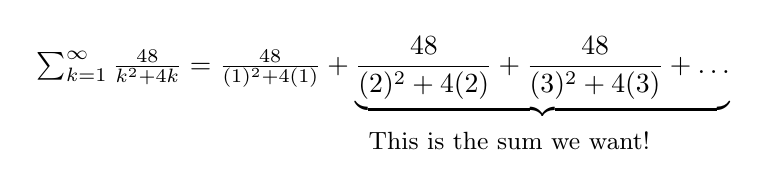
\begin{tikzpicture}
        \node at (0,0) {
          $\sum_{k=1}^{\infty} \frac{48}{k^2+4k}=\frac{48}{(1)^2+4(1)} + \underbrace{\frac{48}{(2)^2+4(2)}+ \frac{48}{(3)^2+4(3)} + \ldots}$};
        \node at (1.6,-.8) {\small{This is the sum we want!}};
      \end{tikzpicture}
  \end{image}
  
  Thus:
  
  \[
  \answer{25} = \answer{\frac{48}{5}} +\sum_{k=2}^{\infty}  \frac{48}{k^2+4k}
  \]
\end{hint}

\end{exercise}


\end{document}
